\documentclass{standalone}
%
\usepackage{tikz,xcolor}
\usetikzlibrary{shapes.geometric,arrows,positioning,fit}
\tikzstyle{arrow} = [thick,->,>=stealth]

\begin{document}
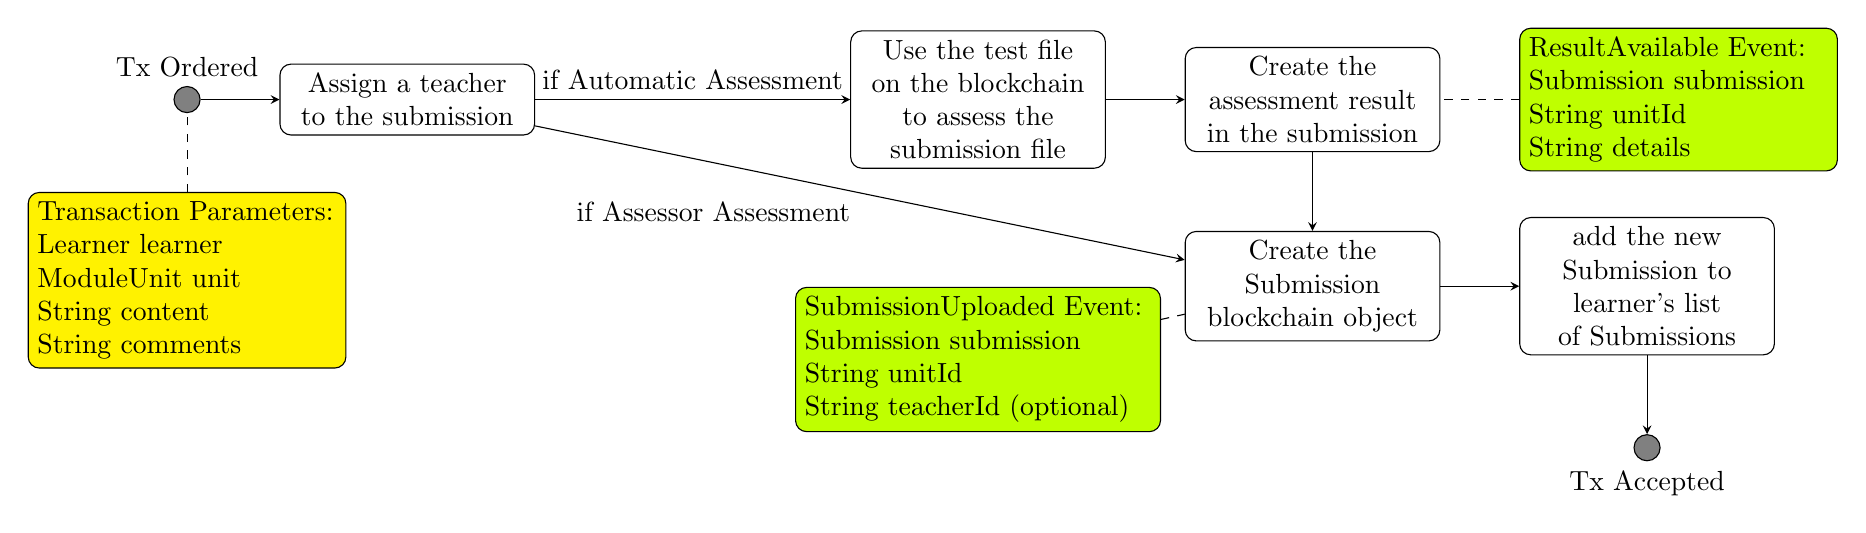
\begin{tikzpicture}[>=stealth,every node/.style={shape=rectangle,draw,rounded corners},]
    % create the nodes
    \node (start)[shape=circle, fill=gray, label=above:Tx Ordered] {};
    \node (param)[below =of start, text width=3.8cm, fill=yellow]{Transaction Parameters:\\Learner learner\\ModuleUnit unit\\String content\\String comments};    
    \node (c1) [right = of start, text width=3cm, align=center]{Assign a teacher to the submission};
    \node (auto1) [right = 4cm of c1, text width=3cm, align=center]{Use the test file on the blockchain to assess the submission file};
    \node (auto2) [right =of auto1, text width=3cm, align=center]{Create the assessment result in the submission};
    \node (event1)[right =of auto2, text width=3.8cm, fill=lime]{ResultAvailable Event:\\ Submission submission\\String unitId \\ String details };
    \node (ass1) [below =of auto2, text width=3cm, align=center]{Create the Submission blockchain object};
    \node (ass2) [right =of ass1, text width=3cm, align=center]{add the new Submission to learner's list of Submissions};
    \node (event2)[below = 1.5cm of auto1, text width=4.4cm, fill=lime]{SubmissionUploaded Event:\\ Submission submission\\String unitId \\ String teacherId (optional) };    
    \node (stop2)[below = of ass2, shape=circle, fill=gray, label=below:Tx Accepted] {};    
    % connect the nodes
    \draw[dashed] (param) to (start);    
    \draw[dashed] (event1) to (auto2);    
    \draw[dashed] (event2) to (ass1);        
    \draw[->] (start) to (c1);
    \draw[->] (c1) -- node[draw=none, anchor=south] {if Automatic Assessment} (auto1);
    \draw[->] (auto1) to (auto2);  
    \draw[->] (auto2) to (ass1);          
    \draw[->] (c1) -- node[draw=none, anchor=north east] {if Assessor Assessment} (ass1);
    \draw[->] (ass1) to (ass2);
    \draw[->] (ass2) to (stop2);    
\end{tikzpicture}
\end{document}
